% asr-gate: certified transcription triage on Aishell-1.
% Primary venue: IEEE/ACM Transactions on Audio, Speech and Language Processing
% (TASLP; SCIE, rolling, ScholarOne). Drafted content-first in article class;
% port to IEEEtran (double column) at submission -- see VENUE-FIT-2026-07-10.md.
% Journal-agnostic article class (reliability-commons paper-template pattern).
% Build: `make paper` (python3 compute_numbers.py -> results/numbers.json;
%   python3 figures/make_figures.py -> figures/fig{1..5}*.pdf; make bib; latexmk).
% Every number below traces to results/numbers.json, which reads only frozen
% result JSONs under ../main_results_2026-07-09 and ../expansion_results_2026-07-09.
\documentclass[11pt]{article}

\usepackage[utf8]{inputenc}
\usepackage[T1]{fontenc}
\usepackage[margin=1in]{geometry}
\usepackage{amsmath,amssymb}
\usepackage{graphicx}
\usepackage{booktabs}
\usepackage{siunitx}
\usepackage{caption}
\usepackage{subcaption}
\usepackage[numbers,round]{natbib}
\usepackage[hidelinks]{hyperref}
\usepackage{xcolor}
\usepackage{authblk}
\usepackage{microtype}
\usepackage{placeins}
\usepackage{cleveref}

\graphicspath{{figures/}}
\captionsetup{font=small,labelfont=bf}
\setlength{\parskip}{0.4em}

\newcommand{\cer}{\mathrm{CER}}
\newcommand{\accset}{\mathcal{A}}

\title{\textbf{Certified Transcription Triage: a Distribution-Free Accept/Defer
Gate with an Audited Confidence Signal for Mandarin ASR}}
\author{Zeyu Fu\thanks{ORCID: \href{https://orcid.org/0009-0001-8329-0108}{0009-0001-8329-0108}.
  Correspondence: \href{mailto:fuzeyu99@126.com}{fuzeyu99@126.com}.
  \textbf{TODO-USER:} affiliation unknown at draft time --- insert department,
  institution, city, and country before submission.}}
\affil{TODO-USER: Institution / Department, City, Country}
\date{\today}

\begin{document}
\maketitle

\begin{abstract}
\noindent Automatic speech recognition (ASR) is increasingly deployed with a human
in the loop, auto-accepting confident transcriptions and deferring the rest. This
raises two questions: can we certify, distribution-free, that the character
error rate (CER) of the auto-accepted set stays below a target, and do field-standard
confidence scores beat honest random deferral? We present a distribution-free accept/defer gate that
(i) issues a Learn-then-Test selective-risk certificate on the accepted-set macro-CER
and (ii) audits each score's excess area-under-the-risk--coverage-curve against an
analytic random-deferral baseline under a matched-abstention permutation null with
Holm control. On Aishell-1 (Paraformer) the certificate holds at $\alpha=2\%$,
$\delta=0.1$ with 0/20 violations across 20 correlated reseeds of one fixed
test set (not 20 independent trials), at $85.7$--$96.2\%$ acceptance and accepted-set
macro-CER $1.00$--$1.53\%$ (full-set $1.98\%$); the binding sub-base-rate target is
$\alpha=1.9\%$ (certified in all 20 reseeds; $\alpha=1.5\%$ is reachable only with a
larger calibration budget, so we report it as budget-conditional). A frozen backbone
$\times$ corpus landscape (three backbones spanning three architectures $\times$ three
credential-free Mandarin corpora) breaks the single-cell reading: a
\emph{documented-open-data} backbone (Belle-whisper, a different architecture and
organization, training data excluding the test) also certifies non-vacuously on the
Aishell-1 test split ($\alpha=5\%$, 0/20), which bounds the undisclosed-training-data
contamination concern by architectural and organizational independence rather than by
assertion; a fully-open transducer failed to expose usable posteriors and is reported
non-certifying (verdict-symmetric). It degrades gracefully under noise and fails
informatively: a weak Whisper zero-shot backbone and a cross-lingual English arm
(LibriSpeech) are honestly vacuous at tight targets, the English certificate holding at
$\alpha=5\%$ on the frozen carve. In the audit, all twelve cells of a roster-derived
family show positive excess area ($0.012$--$0.051$) with speaker-blocked bootstrap 95\%
CIs excluding zero, and the named confidence baselines (class-probability, path
probability, a learned CEM) coincide with our scores to within $\pm0.002$ excess-AURC:
the contribution is the certificate, not a new score. All numbers reproduce from frozen
result files.
\end{abstract}

% On IEEEtran conversion, replace the block below with
% \begin{IEEEkeywords} ... \end{IEEEkeywords}.
\vspace{0.3em}
\noindent\textbf{Index Terms---}speech recognition, conformal risk control, selective
prediction, error-rate certification, distribution-free calibration.

\section{Introduction}\label{sec:intro}

A practical ASR deployment rarely needs every utterance transcribed
automatically; it needs the accepted utterances to be reliable and the
rest routed to a human. This is a selective-prediction problem on a sequence
output --- the modern instance of the classical error/reject tradeoff
\citep{chow1970reject}, whose risk-coverage curve was formalized for learned
classifiers by \citet{elyaniv2010foundations} and later integrated end-to-end
into deep networks \citep{geifman2017selective,geifman2019selectivenet,jones2021selective}
--- and it raises a guarantee question the field-standard confidence pipeline does not
answer: if we auto-accept every utterance whose confidence exceeds a threshold,
what can we promise about the error rate of what we accepted? A promise that is
\emph{distribution-free} --- valid without modeling the error distribution --- is
exactly what conformal risk control provides in other settings
\citep{angelopoulos2022crc,bates2021rcps,angelopoulos2023conformal}.

We make two claims and support each with an independent body of evidence.

\textbf{(C1) Certified selective triage.} The proposed gate certifies, at
preregistered target $\alpha$ on CER and confidence level $1-\delta$, that the
auto-accepted set's macro-CER is at most $\alpha$, at non-trivial coverage on
Aishell-1 test, with an empirical violation rate over 20 calibration reseeds at
most $\delta$. The estimand --- selective risk --- is \emph{non-monotone} in the
threshold, so plain conformal risk control for monotone losses
\citep{angelopoulos2022crc} does not apply; we use Learn-then-Test
\citep{angelopoulos2021ltt} on a reformulated bounded-mean statistic
(\cref{sec:g1}).

\textbf{(C2) A debunk-or-confirm audit.} Field-standard ASR confidence scores
\citep{li2021confidence} either do or do not beat honest random deferral. We test
each score's excess area-under-the-risk-coverage-curve (excess-AURC) against an
analytic random-deferral baseline under a matched-abstention permutation
null, with Holm control over a preregistered, roster-derived family. Both
outcomes publish: ``no confidence signal helps on strong modern ASR'' would be as
informative as the confirmation we in fact observe. Beating random deferral is a
\emph{floor} --- a necessary check that a score is not pure noise, not a claim of
optimality against a calibrated or learned selector; we add temperature-calibrated
($s_5$) and learned-regressor ($s_6$) comparators in \cref{sec:comparator}.

\textbf{Novelty positioning (stated verbatim, because it is load-bearing).}
Conformal prediction for ASR is not new: \citet{ernez2023conformal} control
WER over sentence \emph{prediction sets} and flag uncertain words with inductive
conformal prediction on LibriSpeech/wav2vec\,2.0. Their object is a set of
hypotheses per utterance; ours is an accept/defer \emph{decision} per utterance
with a population-level bound on the accepted set's risk and an explicit
coverage/answered-rate trade-off. We claim novelty only for (i) the audit of ASR
confidence against an analytic random-deferral excess-AURC null (the
selective-classification debunking lens of \citet{traub2024selective}, ported to
sequence output); (ii) a certified accept/defer gate on accepted-set CER for ASR;
and (iii) the released tool. We do not claim ``conformal ASR.'' We also
position against the concurrent generic machinery for non-monotone risk control
\citep{angelopoulos2026nonmonotone} and adaptive selective certificates
\citep{yu2026joint}, and against the 2025--26 selective-risk-control line most adjacent
to ours: \citet{xu2025scrc} and \citet{bai2026conformalselective} develop
general selective/conformal risk control (select-then-control and general-risk
selective prediction) at the abstract-estimand level; \citet{jia2025coverageser} is the
nearest speech-domain instance (coverage-guaranteed \emph{speech-emotion} prediction
sets, a classification output, not sequence-CER); and \citet{zhou2026falsesafety}
audits exactly the bound-tightness and exchangeability strain we concede in the
selective-signal-classification setting. A parallel line applies conformal or
risk-controlling machinery directly to sequence-generating models rather than to a
fixed-vocabulary classifier: \citet{quach2024conformallm} calibrate a stopping/rejection
rule over sampled language-model outputs, \citet{mohri2024conformalfactuality} back off
an LM's claims under a conformal factuality guarantee, and \citet{farinhas2024nonexchangeable}
extend conformal risk control to non-exchangeable sequence data (machine translation) ---
exactly the exchangeability strain we audit empirically via reseeds rather than assume
away (\cref{sec:setup}). These target open-ended text generation or translation; ours
targets a fixed decode's accept/defer decision on CER, a narrower and, we argue, more
auditable target for a production ASR triage gate. These are methods and diagnoses we could
consume, not competitors --- our contribution is the ASR-specific instantiation on
accepted-set CER, the random-deferral audit, and the Mandarin/CER evidence, not new
statistical machinery beyond the LTT layer. This is deliberately an
\emph{application-and-evaluation-protocol} contribution: the novelty is the ASR-specific
instantiation and a reusable evaluation protocol (analytic random-deferral excess-AURC,
matched-abstention permutation null, speaker-blocked bootstrap, and a disclosed-deviation
discipline), and we calibrate the novelty claim accordingly.
\Cref{fig:overview} summarizes the certified transcription-triage pipeline end-to-end.

\begin{figure}[t]
  \centering
  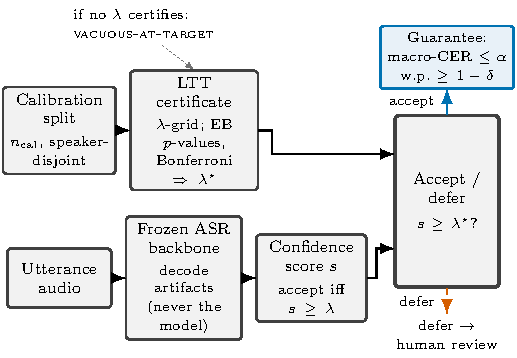
\includegraphics[width=0.53\linewidth]{fig0_overview.pdf}
  \caption{Certified transcription-triage pipeline. Decode artifacts from a frozen ASR
  backbone (never the model itself) yield a per-utterance confidence score
  $s$ (e.g.\ $s_1,s_2$); a speaker-disjoint calibration split ($n_{\mathrm{cal}}$)
  drives Learn-Then-Test construction of a
  threshold $\lambda^\star$ (empirical-Bernstein $p$-values with a Bonferroni-over-grid
  selective-risk procedure) certifying, with probability at least
  $1-\delta$, that the accepted set's macro-CER does not exceed $\alpha$;
  each utterance is then accepted ($s\ge\lambda^\star$) or deferred to a
  human. If no threshold on the grid certifies, the gate reports
  \textsc{vacuous-at-target} rather than accepting nothing silently.}
  \label{fig:overview}
\end{figure}

\section{Method: certified transcription triage}\label{sec:method}

The gate consumes decode artifacts (an $N$-best list per utterance with
sequence log-probabilities and, where available, per-token posteriors) and never
the model itself, so the same gate applies to any backbone that emits those
artifacts. All statistics come from an in-house reliability-metrics library; the
tool ``never computes anything the evaluation did not audit.''

\subsection{Estimand and the loss}\label{sec:estimand}

The per-utterance loss is the character error rate, clipped to $[0,1]$ (insertions can
exceed 1; the clip frequency is reported and is
$0$ on Aishell-1 test):
\begin{equation}
  \ell_i
  = \min\Bigl(1,\;
    \frac{\mathrm{editdist}(\mathrm{hyp}_i,\mathrm{ref}_i)}
         {\mathrm{len}(\mathrm{ref}_i)}\Bigr).
  \label{eq:cer-loss}
\end{equation}
We certify the \emph{macro}-CER (per-utterance mean) of
the accepted set. We separately report the field-standard \emph{micro}-CER
(total edits over total reference characters) with a speaker-blocked bootstrap
confidence interval, but we do not certify it: a micro-CER certificate would
need a length-weighted LTT variant, which we flag as future work. This macro/micro
distinction is stated once here and carried in every table (\cref{tab:cert}). CER is
the natural word-free loss for Mandarin, where segmentation is ambiguous; for
word-segmented languages the same certificate would instead target WER, and
system-independent WER estimation without gold references remains an active
research problem \citep{park2024wer}. This exact, reference-based $\ell_i$ also
differs from reliability-oriented ASR metrics that score the informativeness/error-aversion
trade-off directly, such as RAS \citep{huang2026ras}, which calibrates that trade-off to
human preference rather than certifying a finite-sample risk bound.

\subsection{G1: the selective-risk certificate}\label{sec:g1}

Let $s$ be a confidence score (higher is more confident) and accept iff $s\ge\lambda$.
The selective risk
\begin{equation}
  R(\lambda)
  = \frac{\mathbb{E}[\ell\,\mathbf{1}\{s\ge\lambda\}]}
         {\mathbb{E}[\mathbf{1}\{s\ge\lambda\}]}
  \label{eq:selective-risk}
\end{equation}
is a ratio of two means and is \emph{not monotone} in $\lambda$, so plain conformal
risk control does not give the C1 statement. We use Learn-then-Test
\citep{angelopoulos2021ltt}. The key reformulation: because $R(\lambda)$ is a ratio,
its Hoeffding--Bentkus $p$-value is not computed on $R(\lambda)$ directly. The
per-$\lambda$ null $H_0\!:\,R(\lambda)>\alpha$ is tested through the equivalent
bounded-mean statistic
\begin{equation}
  \mathbb{E}[(\ell-\alpha)\mathbf{1}\{s\ge\lambda\}]>0,
  \label{eq:bounded-mean}
\end{equation}
whose
summand lies in $[-\alpha,\,1-\alpha]$; the two nulls coincide whenever the
acceptance probability is positive. We test a grid of $\lambda$ and select the most
permissive rejected threshold $\lambda^\star$, then accept an utterance iff
$s\ge\lambda^\star$. With probability at least $1-\delta$
over the calibration draw, the accepted set's macro-CER is at most $\alpha$.
Risk--coverage plots report empirical estimates of \eqref{eq:selective-risk} against
coverage $\mathbb{E}[\mathbf{1}\{s\ge\lambda\}]$. We fix
$\delta=0.1$ and certify targets $\alpha\in\{1,2,3,5\}\%$.

\textbf{Disclosed pivot: HB\,$\to$\,EB\,$+$\,Bonferroni (a power fix, with the pilot
trace).} The preregistered pilot used fixed-sequence testing with Hoeffding--Bentkus (HB)
$p$-values. On the same cached pilot calibration data the two procedures give
opposite verdicts at $\alpha=2\%$, side by side: HB certifies nothing (no
threshold rejects, despite an accepted-region CER of $0.95\%$, well under target), whereas
empirical-Bernstein (EB) $p$-values \citep{maurer2009empirical} under a Bonferroni-over-grid
correction certify $\alpha=2\%$ at $86\%$ acceptance. This is a power failure of HB, not a
validity failure: HB bounds the deviation using only the fixed $[0,1]$ range of the
per-$\lambda$ statistic, while EB adapts to its (tiny) sample variance, and for bounded means
EB is \emph{a priori} at least as powerful. Both procedures are finite-sample valid, so
choosing the more powerful valid one is a power upgrade, not a type-I-error risk --- even
though the choice was informed by pilot data. We therefore froze the Bonferroni-over-grid
procedure with EB $p$-values before touching the test set, and we disclose both
outcomes here (HB the conservative preregistered bound, EB the adopted one) --- the deviation
is outcome-visible either way --- rather than presenting only the final procedure.
% frozen config knobs: procedure=bonferroni, p_value=eb

\subsection{G2 and the audit}\label{sec:audit}

The tool also implements a secondary per-utterance split-conformal upper bound (G2),
which we do not evaluate separately here (future work), and a \emph{duration-tercile
Mondrian} stratification of the gate thresholds. The reported certificate throughout
this paper is the G1 selective-risk certificate; its conditional coverage across the
Mondrian duration terciles is reported in \cref{sec:mondrian}.

The audit asks whether a score beats honest random deferral. For each score
we compute its risk--coverage curve, its AURC, and the analytic random-deferral
AURC (closed-form, the risk of accepting a uniformly random subset at each coverage).
The excess-AURC is the area gain
\begin{equation}
  \Delta_{\mathrm{AURC}}(s)
  = \mathrm{AURC}_{\mathrm{rand}} - \mathrm{AURC}(s),
  \label{eq:excess-aurc}
\end{equation}
so $\Delta_{\mathrm{AURC}}(s)>0$ means the score's risk--coverage curve lies below analytic
random deferral. Significance is a matched-abstention permutation
test evaluated at a single operating point --- the score's median accept/defer split
(the top $\lceil n/2\rceil$ utterances by score accepted). The test statistic is the
accepted-set mean CER; the null re-draws which utterances are deferred while holding the
abstention count fixed (within strata when present), preserving the answered rate, and
the one-sided $p$-value is the fraction of $n_{\mathrm{perm}}=2000$ permutations whose
accepted-set mean CER is at most the observed value (floor
$1/(n_{\mathrm{perm}}{+}1)\approx5.0\times10^{-4}$). This median-split permutation $p$ is
a single-operating-point companion to the curve-level excess-AURC statistic, not a
re-test of the same quantity. Family-wise error across the score roster is controlled
with the Holm procedure \citep{holm1979simple}.

\textbf{The multiplicity family is roster-derived, and $m$ is recomputed from what
actually ran (preregistered).} The design specified $m=10$ (5 scores $\times$ 2
backbones). The preregistered recomputation rule states that ``the audit family $m$
is computed from the realized roster after decode gates pass --- one test per
(auditable score, backbone, condition) actually present with $\ge99\%$ non-null
values.'' In the main run only Paraformer's $s_1$ (length-normalized log-posterior)
and $s_2$ (weakest link) survived --- Paraformer exposes no $N$-best margin ($s_3$) or
full posteriors ($s_4$), and the standalone audit never fits the tune-side temperature
for $s_5$ --- so the realized family fell to $m=2$. In the expansion the realized
family is $m=12$: $\{s_1,s_2\}$ on the six (backbone $\times$ condition) cells that
cleared the non-null gate (\cref{sec:results}). The exact $m$ is recorded in each
audit result file and reported with the same denominator everywhere; no $m$ is asserted
in advance.

\subsection{Honest-uncertainty rules}\label{sec:honest}

Out-of-stratum utterances (a stratum with $<200$ calibration utterances) are deferred
unconditionally. A cheap two-stage detector routes non-Mandarin input to a distinct
\textsc{ood-refuse} state (a validity statement, not an uncertainty estimate): on
Aishell-1 test this fires on 3 utterances on every reseed, independent of the gate.
A domain fingerprint stored in the gate warns when an incoming batch's score
distribution shifts beyond a preregistered KS distance (warning only, never silent
recalibration). The gate's calibrate and audit modes refuse to run without references;
its apply mode runs reference-free by design.

\section{Experimental setup}\label{sec:setup}

\textbf{Data.} Aishell-1 \citep{bu2017aishell} is $\sim$178\,h of read Mandarin
(16\,kHz). We use the official test split (20 speakers, 7{,}176 utterances, all
transcribed, 0 empty), and carve the 40-speaker dev split into speaker-disjoint
calibration (20) and tune (20) sets. The cross-corpus arm uses the THCHS-30 test
split \citep{wang2015thchs30} ($n=2{,}495$ utterances --- the full official test split,
the ten D-prefix test speakers --- from the corrected re-decode; the earlier $n=1{,}339$
decode drew from a \emph{mislabeled mirror split} that was mostly train-speaker audio, not
the test split, disclosed below and in \cref{tab:deviations}). The noise arm
mixes ESC-50 environmental audio \citep{piczak2015esc50} additively onto Aishell-1
test at 5/15/25\,dB SNR --- a disclosed substitution for the design's MUSAN, which was
unreachable at usable bandwidth; the mixer is source-agnostic and the SNR
stratification is unchanged. A cross-lingual English arm decodes LibriSpeech
\citep{panayotov2015librispeech} test-clean and test-other with Whisper large-v3 and
two wav2vec\,2.0 checkpoints \citep{baevski2020wav2vec2}, carving test-clean speaker-disjointly (seed~0)
% English wav2vec2 checkpoints: facebook/wav2vec2-base-960h (``base'') and
%   facebook/wav2vec2-large-960h-lv60-self (``large''); both zero-shot CTC.
into a calibration split ($n=1{,}352$; fit~739 $+$ cal~613) and a held-in eval-clean split
($n=1{,}268$), and applying the gate to test-other ($n=2{,}939$) as a shifted split
(\cref{sec:crosslingual}). \Cref{tab:data} gives the full spec.
% source: THCHS n=2495 = line count of
%   results/expansion/scored/thchs30_whisper_scored_fixed_2026-07-12.jsonl (full official
%   test, ten D-prefix speakers; the aggregate redecode-delta JSON was not archived, so the
%   per-utterance scored file is the source of record). English-arm splits from
%   ../english_arm_fixed_2026-07-12/ATTAINMENT.json (n) + ../english_arm_fixed_2026-07-12/
%   gate_whisper_a0.05.json (n_fit=739, n_cal=613); test-clean carve = 739+613+1268=2620.

\textbf{Backbones.} We attempted three released checkpoints, zero-shot (no training):
Paraformer \citep{gao2022paraformer,gao2023funasr} (the primary certified backbone),
Whisper large-v3 \citep{radford2023whisper} (zero-shot Mandarin, an out-of-domain
stressor), and a ModelScope Conformer-Aishell checkpoint (replacing the design's
WeNet backbone \citep{yao2021wenet}, which had no installable wheel for the run environment). The Conformer
checkpoint emits tokens and text but \emph{no per-token posteriors}, so $s_1,s_2$ are
uncomputable; per the honest-uncertainty rule it is recorded as
\textsc{skipped-degraded} and excluded from the audit and certificate --- never
imputed. This is why the realized roster spans Paraformer and Whisper only.

\textbf{Reseeds instead of training seeds.} No training occurs, so we resample the
dev$\to$cal/tune carve at the speaker level 20 times (seeds 0--19), decoding once and
recalibrating on cached scores. The empirical violation rate over these 20 reseeds is
the primary validity evidence for C1.

\textbf{Exchangeability candor (load-bearing).} Utterances within a speaker are not
independent; speaker is the natural block. Cal/tune/test are speaker-disjoint by
construction, and all reported CIs are speaker-blocked bootstraps (block $=$ speaker;
$\sim$40 dev / 20 test blocks). The LTT/G2 guarantees assume utterance-level
exchangeability between calibration and test, which speaker-level dependence and
cal-vs-test speaker disjointness both strain; the 20-reseed violation rate is our
direct empirical check on that assumption, and the 20-block test-side bootstrap gives
deliberately wide intervals rather than false precision. We state this in the body,
not an appendix.

\textbf{Disclosed protocol deviations} are collected in \cref{tab:deviations}: the
WeNet$\to$Conformer(degraded) roster change, the HB$\to$EB$+$Bonferroni pivot, the
ESC-50-for-MUSAN and THCHS-mirror substitutions, and the roster-derived $m$
($10\to2$ main, $12$ expansion). Data-integrity carry-forward: 17 zero-frame wavs
(2 dev / 15 train / 0 test) skipped and logged; 4/7{,}176 test utterances (0.056\%)
with degraded token-logp extraction, excluded-and-counted per score. A separate
data-integrity anomaly surfaced in the cross-corpus arm, and its accurate mechanism is a
\emph{wrong evaluation pool}, not a truncation: the original THCHS-30 decode ($n=1{,}339$,
59 speakers, zero duplicate utterances) drew from a mislabeled mirror split that was
$82.7\%$ train-speaker audio (1{,}107 of 1{,}339 utterances from train/dev speakers),
with only $232$ utterances from the genuine test split. Two things are therefore
conflated in the old number and we separate them. (i) \emph{Pool change:} the aligned
re-decode on the correct full official test split ($n=2{,}495$, the ten D-prefix test
speakers) reports full-set macro-CER $9.93\%$, versus $15.77\%$ on the contaminated
$1{,}339$-utterance mirror pool. (ii) \emph{Like-for-like:} restricted to the $232$
utterances that are genuine test utterances in both decodes, macro-CER falls from
$16.27\%$ to $9.72\%$ ($6.55$~pp), a paired comparison that isolates the decode fix from
the pool change. We disclose the wrong-pool contamination and report the corrected
test-split number for the Whisper cross-corpus audit cell (\cref{tab:cert,tab:holm}) rather
than silently swapping it. The backbone-landscape THCHS-30 cells (\cref{tab:landscape},
all three backbones) were originally computed on the same $1{,}339$-utterance mirror pool;
they have since been re-decoded on the corrected $n{=}2{,}495$ official test (2026-07-16,
\cref{tab:deviations}), so \cref{tab:landscape} and the Whisper audit cell now both report
the official-pool numbers.
% source: verified from the two shipped THCHS files against the official split listing
%   (libri_staging/data_thchs30/{train,dev,test}); reproduced numbers:
%   original results/expansion/scored/thchs30_whisper_scored.jsonl (n=1339, 59 spk, 0 dup;
%   1107/1339=82.67% train/dev-speaker; 232 genuine test utts; full-set macro-CER 0.15766;
%   232-utt macro-CER 0.16267), fixed results/expansion/scored/
%   thchs30_whisper_scored_fixed_2026-07-12.jsonl (n=2495 full official test; full-set
%   macro-CER 0.09931; same 232 utts 0.09717). 15.77/9.93/16.27/9.72 all trace here.


\begin{table}[h]
  \centering
  \caption{Dataset and split specification. Every backbone gate calibrates on a
  speaker-disjoint carve of the Aishell-1 dev split; each test split is the official
  split, touched once. THCHS-30, MagicData, and the ESC-50 noise mixes are apply/audit-only
  (calibration always stays on Aishell dev, so the Mandarin cross-corpus cells are transfer
  cells). The three landscape backbones (Paraformer, Belle, zipformer) each decode the three
  Mandarin test splits in the certified landscape.}
  \label{tab:data}
  \small
  \begin{tabular}{l p{0.24\textwidth} r p{0.24\textwidth}}
    \toprule
    Corpus & Role & Utterances & Notes \\
    \midrule
    Aishell-1 dev  & cal (20 spk) + tune (20 spk) & 14{,}326 & speaker-disjoint carve \\
    Aishell-1 test & certify + audit (3 backbones) & 7{,}176 & official, touched once \\
    Aishell-1 test + ESC-50 & noise robustness (Para.) & 7{,}176 & additive 5/15/25\,dB SNR \\
    THCHS-30 test  & cross-corpus audit cell (Whisper) + transfer landscape (3 backbones) & 2{,}495 & full official test (ten D-prefix spk); corrected re-decode (disclosed pool fix) \\
    MagicData test & cross-corpus transfer (3 backbones) & 4{,}094 & CC BY-NC-ND; speaker-disjoint $\sim$4k cap; disclosed SLR62$\to$MagicData substitution \\
    LibriSpeech test-clean & English cal (739$+$613) $+$ eval-clean & 2{,}620 & English arm; speaker-disjoint carve \\
    LibriSpeech test-other & English cross-lingual apply & 2{,}939 & English arm; shifted split \\
    \bottomrule
  \end{tabular}
\end{table}
% source: THCHS n=2495 = Whisper audit cell (line count of results/expansion/scored/
%   thchs30_whisper_scored_fixed_2026-07-12.jsonl, corrected official test) AND the
%   landscape 3-backbone cells (../thchs_official_pulled_2026-07-16/
%   decode_thchs30_official_{paraformer,belle,zipformer}.jsonl, 2495 lines each; official
%   D-prefix test re-decode 2026-07-16, see tab:deviations) -- both now on the same
%   n=2495 official pool, so the two former THCHS rows are merged; LibriSpeech test-clean 2620 =
%   1352 cal (739 fit + 613 cal) + 1268 eval-clean; test-other 2939
%   (../english_arm_fixed_2026-07-12/ATTAINMENT.json).

\begin{table}[h]
  \centering
  \caption{Disclosed protocol deviations from the design and freeze note. Each was
  fixed before the test set was touched, except the roster-derived $m$ (computed from
  realized decodes by preregistered rule) and the MagicData eval cap (applied post-hoc to
  cached scores, by the rule frozen ahead of the decode).}
  \label{tab:deviations}
  \small
  \begin{tabular}{p{0.30\textwidth}p{0.62\textwidth}}
    \toprule
    Deviation & Disposition \\
    \midrule
    WeNet backbone $\to$ Conformer-Aishell & no installable wheel; Conformer then \textsc{skipped-degraded} \\
    Conformer-Aishell in the audit & no per-token posteriors $\Rightarrow$ $s_1,s_2$ null $\Rightarrow$ excluded \\
    Hoeffding--Bentkus $\to$ EB $+$ Bonferroni & pilot power failure (certified nothing at $\alpha{=}2\%$); disclosed \\
    MUSAN noise $\to$ ESC-50 & MUSAN unreachable at bandwidth; source-agnostic mixer \\
    THCHS-30 openslr $\to$ parquet mirror & delivery-route substitution; corrected pool is the full official test ($n{=}2{,}495$, ten D-prefix speakers) \\
    THCHS-30 original decode was the wrong pool & the $n{=}1{,}339$ mirror split was $82.7\%$ train-speaker audio (59 spk, 0 dup), only 232 genuine test utts; corrected to the official test, macro-CER $15.77\!\to\!9.93\%$ (232-utt like-for-like $16.27\!\to\!9.72\%$) \\
    THCHS-30 landscape cells re-decoded on the official test (done 2026-07-16) & the backbone-landscape THCHS-30 cells (all three backbones) were originally computed on the $n{=}1{,}339$ mislabeled mirror pool; they were re-decoded on the corrected $n{=}2{,}495$ official test (ten D-prefix speakers) on 2026-07-16, and the landscape table now reports the official-pool numbers. The historical mirror-pool cells are retained frozen but superseded; both THCHS-30 arms (this landscape and the Whisper audit cell) are therefore on the same official test \\
    aidatatang (SLR62) $\to$ MagicData (SLR68) & SLR62 withdrawn upstream on launch day (two networks); MagicData was the amendment's frozen optional 4th corpus, substituted with no other frozen change \\
    MagicData eval cap (post-hoc) & the full $\sim$24k test was decoded; the frozen speaker-disjoint $\sim$4k cap (9 spk, $n{=}4{,}094$) was applied post-hoc to the cached scores at eval/audit and disclosed \\
    Holm family size $m$ & roster-derived: design 10, main run 2, expansion 12; landscape audit cells recompute $m$ (2 where $s_1,s_2$ present) \\
    Gender Mondrian axis & dropped: decode records carry no gender label (future work) \\
    \bottomrule
  \end{tabular}
\end{table}

\section{Results}\label{sec:results}

Every number in this section is read from archived experimental artifacts, computed
only from those frozen records; every figure regenerates from them.
% single number-registry file: results/numbers.json (from compute_numbers.py)

\subsection{The certificate holds on clean Aishell-1 (C1)}

\Cref{fig:teaser} shows the $s_1$ risk--coverage curve on test: the gate tracks well
below the analytic random-deferral line and approaches the oracle. Across 20
speaker-level reseeds at $\alpha=2\%$, $\delta=0.1$, the certificate holds with
0/20 violations, acceptance fraction $85.7$--$96.2\%$ (mean $90.7\%$), and
accepted-set macro-CER $1.00$--$1.53\%$ (mean $1.21\%$; accepted-set micro-CER
$1.02$--$1.54\%$, mean $1.23\%$) --- against a full-set
macro-CER of $1.98\%$, so the gate cuts the error rate by roughly $40\%$
($1.98\%\!\to\!1.21\%$ mean) on the accepted $\sim$91\% of traffic.
% source: accepted-set macro from numbers.json (main_attainment accepted_cer_min/max/mean);
%   accepted-set micro companion from results/accepted_micro_2026-07-13.json (descriptive,
%   not certified; macro cross-checks the frozen 1.00-1.53/1.21).
\Cref{fig:frontier} gives the certified frontier: $\alpha=1\%$
is \textsc{vacuous-at-target} (dev macro-CER already exceeds 1\%, so no threshold
certifies and 0\% is accepted --- reported, not silently dropped); $\alpha=3\%$ and
$\alpha=5\%$ both certify at $99.8\%$ coverage (a grid-floor saturation: the most
permissive candidate already satisfies both budgets). The inset shows the
$0/20$ violation count against the $\delta=0.1$ line.

\begin{figure}[t]
  \centering
  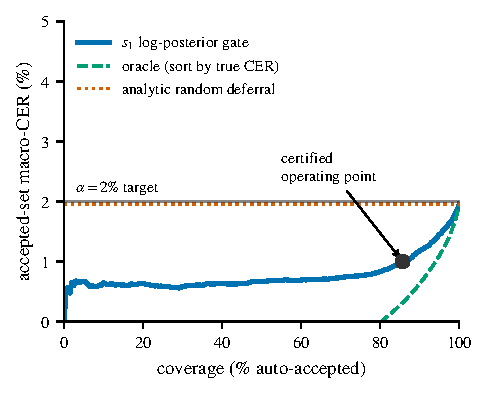
\includegraphics[width=0.50\linewidth]{fig1_teaser_rc.pdf}
  \caption{Risk--coverage on Aishell-1 test (Paraformer, $s_1$): the confidence gate
  (blue) tracks well below the analytic random-deferral line (dotted) and approaches
  the oracle (dashed). The marked operating point is reference reseed~0 (the
  minimum-acceptance reseed): it auto-accepts 85.7\% of utterances at 1.00\% macro-CER,
  under the $\alpha{=}2\%$ target; the mean over 20 reseeds is 90.7\% acceptance.
  (The dotted random-deferral asymptote is the $s_1$-audit-subset macro-CER, $1.95\%$
  over the $n{=}7{,}172$ utterances with a non-null $s_1$; the $1.98\%$ full-set figure
  (The dotted random-deferral asymptote is the $s_1$-audit-subset macro-CER, $1.95\%$
  over the $n{=}7{,}172$ utterances with a non-null $s_1$; the full-set macro-CER
  $1.98\%$ is over all $n{=}7{,}176$ utterances --- hence the $1.95$ vs $1.98\%$ hair.)}
  \label{fig:teaser}
\end{figure}

\begin{figure}[t]
  \centering
  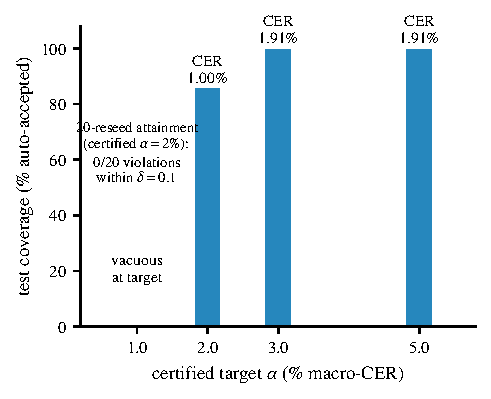
\includegraphics[width=0.51\linewidth]{fig3_certified_frontier.pdf}
  \caption{Certified frontier (Paraformer test), at reference reseed~0 (the
  minimum-acceptance reseed; the 20-reseed mean acceptance at $\alpha{=}2\%$ is 90.7\%).
  $\alpha{=}1\%$ is \textsc{vacuous-at-target} (0\% acceptance); $\alpha{=}2\%$ certifies
  at 85.7\% coverage; $\alpha{=}3\%$ and $5\%$ saturate at 99.8\%. The annotation over
  the vacuous $\alpha{=}1\%$ column reports the $\alpha{=}2\%$ certificate's reseed
  attainment: 0/20 violations across the 20 reseeds, within the $\delta{=}0.1$ budget.}
  \label{fig:frontier}
\end{figure}

The certificate's information on clean data is the conditional accepted-set quality
and the binding regimes, not the raw violation count (base-rate disclosure). The full-set
macro-CER on clean Paraformer is $1.98\%$, just under the $2\%$ target, so accept-all already
meets an $\alpha=2\%$ budget and the $\alpha\in\{3,5\}\%$ certificates saturate at accept-all;
what the $\alpha=2\%$ certificate adds is that it does not accept all --- it withholds
the low-confidence tail, certifying a restricted $85.7$--$96.2\%$ set at $1.00$--$1.53\%$
accepted-set macro-CER. Below the base rate the target genuinely binds, and we map that regime
post-hoc by replicating the frozen reseed protocol with only $\alpha$ changed: $\alpha=1.5\%$
is honestly vacuous ($0/20$ certified at the frozen $n_{\mathrm{cal}}\approx3{,}567$), while
$\alpha=1.9\%$ --- below the $1.98\%$ base rate, so accept-all would fail --- certifies in all
$20$ reseeds at $87.8\%$ mean acceptance and $1.09\%$ accepted-set macro-CER, with $0$
violations across the whole $1.5$--$2.0\%$ band. The certificate therefore does non-trivial
work precisely where a budget below the error floor makes accept-all inadmissible.
% source: alpha015_2026-07-13/results.json (binding_band_sweep + summary; frozen main reseed
%   protocol at alpha=1.5-2.0%; delta=0.1 verified in each reseed gate.json).

The $\alpha=1.5\%$ floor is reachable with more calibration budget (post-hoc).
That $\alpha=1.5\%$ vacuity is itself a calibration-budget artifact, not a property of
the bound --- the same effect the English arm exhibits (\cref{sec:crosslingual}). A post-hoc
calibration-size sweep makes this concrete on the Mandarin arm, with a cleaner design than the
English one: we hold the \emph{fixed official test} as eval (calibrating on the speaker-disjoint
dev pool, so there is no test-partition calibration caveat) and vary only $n_{\mathrm{cal}}$.
The flat Learn-then-Test bound (identical machinery to the English sweep) certifies
$\alpha=1.5\%$ non-vacuously once $n_{\mathrm{cal}}$ reaches $\approx5{,}000$, accepting
$83.2\%$ of the fixed test at $0.91\%$ accepted-set macro-CER with $0$ violations, stable in
$4$ of $5$ dev-pool re-draws ($n_{\mathrm{cal}}=7{,}000$ in the fifth). The crossover budget is
monotone in the target ($\alpha{=}1.5\%\!\to\!5{,}000$, $1.7\%\!\to\!3{,}567$,
$1.9\%\!\to\!3{,}000$, $5\%\!\to\!1{,}000$), qualitatively consistent with the
$1/\sqrt{n_{\mathrm{cal}}}$ bound slack. The effect survives the frozen certificate machinery: the main run's
calibration gate (duration-tercile Mondrian) on the full dev pool
($n_{\mathrm{cal}}\approx7{,}184$ after the fit/conformalize split), applied to the same fixed
test, certifies $\alpha=1.5\%$ at $90.6\%$ acceptance and $1.20\%$ accepted-set macro-CER, $0$
violations --- versus $0/20$ certified at the frozen $\approx3{,}567$-carve. With
$\approx5{,}000$ speaker-disjoint dev calibration utterances the certified frontier therefore
tightens from $\alpha=2\%$ to a binding $\alpha=1.5\%$ on the same test data, for $0$ additional
GPU-hours.

\begin{figure}[t]
  \centering
  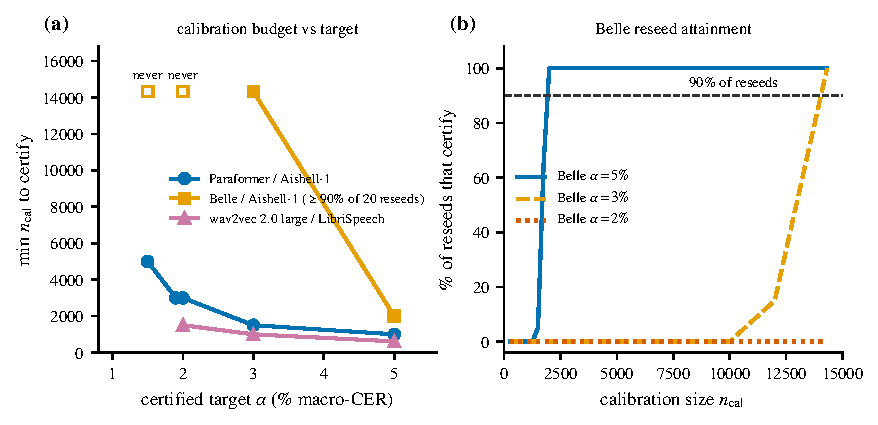
\includegraphics[width=0.92\linewidth]{fig6_calsize_sweep.pdf}
  \caption{Calibration budget versus certified target, from archived calibration-size
  records (no new decoding). (a)~Smallest $n_{\mathrm{cal}}$ at which the accept/defer gate
  certifies non-vacuously: Paraformer and Belle on Aishell-1, and wav2vec 2.0 large on
  LibriSpeech. Open markers sit at the available pool when that target never certifies.
  (b)~Belle: fraction of 20 calibration reseeds that certify at $\alpha=5\%$, $3\%$, and
  $2\%$. The dashed line at $90\%$ is the stability cutoff for the smallest reported
  $n_{\mathrm{cal}}$.}
  \label{fig:calsize}
\end{figure}
% source: mandarin_calsweep_2026-07-13/results.json --- crossover_seed0 (0.015->5000,
%   0.017->3567, 0.019->3000, 0.05->1000) + crossover_seed_robustness[0.015]=[5000,5000,5000,
%   5000,7000] (4/5 at 5000, 7000 in seed 4); cells_seed0 alpha=0.015 @ n_cal=5000:
%   eval_accept_rate=0.831567 (83.2%), eval_accepted_macro_cer=0.0091355 (0.91%),
%   eval_violation=false; frozen_machinery_confirmation alpha=0.015: n_cal=7184, n_fit=7141,
%   eval_accept_rate=0.906023 (90.6%), eval_accepted_macro_cer=0.0120364 (1.20%),
%   eval_violation=false; consistency_guard reproduces_frozen=true (max|ds1|=max|dCER|=0.0 over
%   7,172 utts). Same flat LTT/EB/Bonferroni machinery (delta=0.1, n_grid=200,
%   min_accept_frac=0.1) as english_calsweep_2026-07-13.

\textbf{Interpreting 0/20 against $\delta=0.1$ (a correlated diagnostic, read for
conservatism not calibration).} We are explicit about what this $0/20$ does and does not
establish. The 20 reseeds resample only the calibration/tune carve from a fixed
40-speaker dev pool and apply each resulting gate to the same fixed test set, so
they are 20 strongly correlated draws, not 20 independent $\mathrm{Bernoulli}(\delta)$
trials; we therefore do not read $0/20$ as a $\pm$ error bar on the violation
probability, and it does not certify validity on a fresh test set. What it does
show is that the accepted-set risk stays under $\alpha$ across the calibration
randomness we can resample here, with margin --- an empirically conservative realized
rate consistent with the deliberate conservatism of the LTT bound. A valid,
finite-sample-honest procedure is expected to under-shoot $\delta$; we would worry only
about the reverse (systematic excess), which we do not observe.

\textbf{Adding the speaker-exchangeability axis (post-hoc).} The 20 reseeds vary only the
calibration draw; the eval speaker population is fixed, so they cannot probe speaker-level
variability in what is evaluated. We add that axis directly: repartitioning the full
$60$-speaker Aishell-1 pool (dev $40$ $+$ test $20$) into a $20$-speaker calibration cohort
and a \emph{disjoint} $20$-speaker eval cohort, $R=20$ times, and rerunning calibrate$+$apply
at $\alpha=2\%$, gives $0/20$ violations with the eval speakers themselves changing every
partition, at $86.7$--$95.0\%$ acceptance and $1.00$--$1.38\%$ accepted-set macro-CER
($n_{\mathrm{cal}}$ held at the frozen $\approx3{,}567$ scale) --- ranges essentially
indistinguishable from the calibration-only reseed check. The reseed check thus probes
calibration randomness and the speaker-partition check probes speaker exchangeability; both
pass. This partition check necessarily calibrates on partitions of the official test split, so
we report it as a disclosed post-hoc validity probe, not a headline; the main-run numbers
still calibrate on dev only.
% source: speaker_partition_2026-07-13/results.json (R=20 speaker partitions; 0/20 violations
%   at alpha=2%; acceptance 86.7-95.0%, accepted macro-CER 1.00-1.38%, n_cal 3537-3622).

\subsection{Conditional coverage across duration terciles}\label{sec:mondrian}

The $0/20$ reseed-violation count of the $\alpha=2\%$ Paraformer certificate on Aishell-1
test is a marginal statement. Because the deployed gate is Mondrian in
audio duration --- its threshold is set per duration tercile, with edges frozen on each
reseed's calibration split --- we can ask whether the certificate also holds within
each tercile. \Cref{tab:mondrian} reports, per tercile at $\alpha=2\%$, the acceptance rate,
the accepted-set macro-CER, and the violation count over the 20 reseeds. The certificate
holds conditionally: 0/20 violations in every tercile, and every tercile's
speaker-blocked bootstrap 95\% CI (reference reseed~0) sits below $1.4\%$, comfortably under
the $2\%$ target. The one visible heterogeneity is a mild, expected difficulty gradient: long
utterances (dur2) run about $0.3$~pp higher in accepted-set macro-CER ($1.36\%$ vs
$1.06$--$1.12\%$) and about $2$~pp lower in acceptance ($89.8\%$ vs $91.4$--$91.8\%$) than
short and medium ones, which the Mondrian thresholds absorb by setting a tighter score
threshold on the long tercile (reference reseed~0: $0.111$ for dur2 vs $0.150$ for dur0). This
is a difficulty gradient the per-stratum design anticipates, not a failure of control.

\begin{table}[t]
  \centering
  \caption{Conditional coverage across duration terciles (Paraformer, Aishell-1 test,
  $\alpha=2\%$, 20 reseeds). Tercile edges are frozen on each reseed's calibration split and
  applied to test, so tercile sizes are unequal and reseed-dependent. The certificate holds
  within every tercile (0/20 violations). The 95\% CI is a speaker-blocked bootstrap on the
  reference reseed~0 accepted-set macro-CER (2{,}000 resamples, block $=$ speaker, percentile).}
  % source file: results/mondrian_tercile_analysis.json
  % TABLEFIX-2026-07-16 KEEP-JUSTIFIED (3 data rows, < 5): checked
  %   results/mondrian_tercile_analysis.json for a hidden categorical axis to expand (per the
  %   corrected review-directive guidance preferring expansion over merge/prose) -- it does
  %   carry a per_reseed block (20 reseeds x 3 terciles = 60 raw rows), but reseed index is a
  %   resampling nuisance parameter, not a category like backbone/corpus/class; the table
  %   already reports the correct honest summary of that repeated-measures data (mean/min/max
  %   + violations + CI per tercile), so expanding to 60 raw rows would not surface new
  %   categorical detail, only replace a well-organized summary with a data dump. The row
  %   count is instead fixed by the design's tercile axis (short/medium/long duration
  %   strata) -- there is no fourth stratum to add without inventing an axis (the only other
  %   candidate, gender, is dropped per tab:deviations for lack of a label). No thematically
  %   adjacent table shares this column schema (accept %, acc-CER, violations, CI per
  %   stratum), so no natural merge partner exists either. The surrounding prose already
  %   narrates the qualitative gradient, and this table is the only place the per-tercile
  %   CIs and reseed-min/max ranges appear. Kept as-is.
  \label{tab:mondrian}
  \small
  \setlength{\tabcolsep}{4.5pt}
  \begin{tabular}{llrcc}
    \toprule
    Tercile & Accept.\ \% & Acc.-set CER \% & Viol. & Reseed-0 \\
     & (mean [min, max]) & (mean [min, max]) & & 95\% CI \\
    \midrule
    dur0 / short  & 91.8 [86.8, 96.3] & 1.12 [0.92, 1.40] & 0/20 & $[0.77, 1.09]$ \\
    dur1 / medium & 91.4 [87.0, 96.2] & 1.06 [0.86, 1.33] & 0/20 & $[0.72, 0.97]$ \\
    dur2 / long   & 89.8 [84.1, 96.2] & 1.36 [1.16, 1.75] & 0/20 & $[1.01, 1.32]$ \\
    \bottomrule
  \end{tabular}
\end{table}

\subsection{The certificate degrades gracefully under noise}

\Cref{fig:noise} applies the \emph{clean-calibrated} gate to noisy test audio. At
25\,dB and 15\,dB SNR the certificate holds with $0/20$ violations (accepted-set
macro-CER $1.22\%$ and $1.32\%$, coverage $90.3\%$ and $89.4\%$); at 5\,dB it shows
$1/20$ violations (accepted-set macro-CER $1.62\%$, up to $2.16\%$ on the single
violating reseed, coverage $82.2\%$). One violation in 20 is a realized rate of
$0.05$, still within the $\delta=0.1$ budget: the gate calibrated on clean speech
transfers to moderate noise and begins --- honestly --- to strain only at the most
severe 5\,dB condition (the largest nominal SNR drop, where the distribution shift the
domain fingerprint is meant to flag is plausibly largest).

\begin{figure}[t]
  \centering
  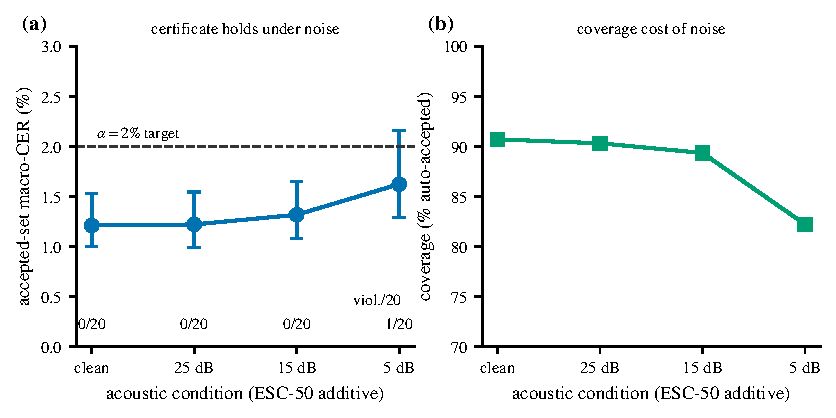
\includegraphics[width=0.86\linewidth]{fig4_noise_robustness.pdf}
  \caption{Noise robustness: the clean-calibrated Paraformer gate applied to ESC-50
  additive noise. (a) Accepted-set macro-CER (error bars: min--max over 20 reseeds) stays
  under the $\alpha{=}2\%$ target with 0/20 violations at 25 and 15\,dB and 1/20 at
  5\,dB (within the $\delta{=}0.1$ budget). (b) Coverage cost of noise: mean auto-accepted
  fraction falls from $90.7\%$ on clean audio to $90.3\%$/$89.4\%$ at 25/15\,dB and
  $82.2\%$ at 5\,dB.}
  \label{fig:noise}
\end{figure}

\subsection{Cross-corpus: the audit transfers where the certificate cannot}

The Whisper zero-shot Mandarin cells are a \emph{deliberately weak-backbone stressor}:
Whisper large-v3 is not tuned for Mandarin, and its full-set macro-CER is $28.1\%$ on
Aishell and $9.93\%$ on THCHS-30 (corrected re-decode, \cref{sec:setup}) ---
far above any certified target. They are included not to certify but to exercise the gate's
vacuity behaviour and to supply audit-informative cells where the certificate cannot hold.
Consequently the Whisper gate is vacuous at every $\alpha\in\{1,2,3,5\}\%$ (0\% acceptance):
% source: 28.1% and 9.93% from tab:cert; 9.93% recomputed in
%   results/expansion/scored/thchs30_whisper_scored_fixed_2026-07-12.jsonl (macro-CER 0.09931, n=2495).
no low-CER accepted region exists to certify (\cref{fig:vacuity} shows the Whisper
curves plateauing well above the $2\%$ ceiling while Paraformer dips below it). Yet
the audit still fires on Whisper (below), cleanly separating the two claims:
confidence can carry selective skill on a backbone too weak to support a low-CER
certificate. This is the design's preregistered vacuity outcome, and it is
verdict-symmetric --- a weak backbone that cannot certify a strong target is a finding,
not a failure.

\begin{figure}[t]
  \centering
  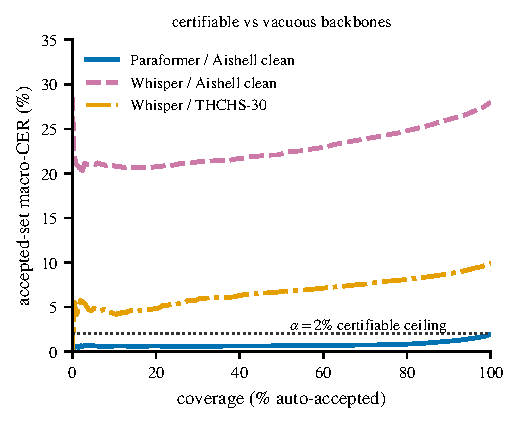
\includegraphics[width=0.53\linewidth]{fig5_vacuity_rc.pdf}
  \caption{Why the certificate is vacuous on weak backbones. Paraformer/Aishell dips
  below the $\alpha{=}2\%$ ceiling (certifiable); Whisper/Aishell and Whisper/THCHS-30
  plateau far above it, so no threshold yields a $\le2\%$ accepted set --- even though
  the audit still finds significant selective skill on these backbones.}
  \label{fig:vacuity}
\end{figure}

\subsection{Cross-lingual: a non-vacuous English certificate at $\alpha=5\%$}\label{sec:crosslingual}

To test whether the certificate transfers beyond Mandarin, we run an English arm on
LibriSpeech with three strong English backbones (Whisper large-v3 and two wav2vec\,2.0
checkpoints, base and the larger LV60k-Self self-trained model),
calibrating on a speaker-disjoint half of test-clean and applying the gate to the held-in
eval-clean split and to the harder test-other split (\cref{sec:setup}). \Cref{tab:english}
reports the outcome at $\alpha=5\%$. The certificate is non-vacuous: it certifies
at $\ge97.99\%$ acceptance with accepted-set macro-CER $0.61$--$3.90\%$, comfortably under
the $5\%$ target, on all three backbones and both splits (certified thresholds
$\lambda^\star=-0.0959$ for Whisper, $-0.1989$ for wav2vec\,2.0 base, and $-0.1498$ for
wav2vec\,2.0 large). On test-other the
domain fingerprint fires a shift warning (KS distance $0.176$ for Whisper, $0.280$ for
wav2vec\,2.0 base, $0.247$ for wav2vec\,2.0 large, all above the $0.15$ warn threshold),
yet the $\alpha=5\%$ bound is still
respected --- the gate flags the shift and holds. At the frozen $613$-utterance
calibration carve the tighter targets are vacuous: at $\alpha\in\{1,2,3\}\%$ every cell
accepts $0\%$, as no threshold clears the distribution-free bound on that carve even on
these strong backbones. This sub-$5\%$ vacuity is a calibration-budget
property, not an intrinsic property of the bound. The Learn-then-Test empirical-Bernstein
bound slack shrinks with the calibration sample size, so the same held-out test-clean
utterances certify tighter targets given more calibration data. A post-hoc calibration-size
sweep --- holding a fixed speaker-disjoint eval set and varying only $n_{\mathrm{cal}}$,
stable across five eval/cal re-draws --- makes this concrete: $\alpha=3\%$ certifies
non-vacuously once $n_{\mathrm{cal}}$ reaches $\approx1{,}500$ on all three backbones
($\approx1{,}000$ on the strongest, wav2vec\,2.0 large, which also has the lowest
accepted-set error --- eval-clean CER $0.61\%$, test-other $1.70\%$), and $\alpha=2\%$
certifies at $n_{\mathrm{cal}}=1{,}500$ on wav2vec\,2.0 large (accepting $96.7\%$ of
eval-clean at $0.42\%$ accepted-set macro-CER, a non-vacuous certificate), while
Whisper and wav2vec\,2.0 base do not reach $\alpha=2\%$ within the $\approx2{,}000$-utterance
test-clean calibration pool. We report this as practitioner guidance --- what calibration
data buys --- rather than a limitation of the bound: the English arm yields a second language
and three backbones under a non-vacuous $\alpha=5\%$ certificate on the frozen carve, with
$\alpha=3\%$ reachable at a realistic calibration budget.
% source: calibration-size sweep english_calsweep_2026-07-13/results.json (crossover n_cal per
%   backbone/alpha; seed-robust over eval/cal re-draws 0-4; frozen LTT/EB/Bonferroni machinery).
% source: ../english_arm_fixed_2026-07-12/ATTAINMENT.json + ../english_arm2_2026-07-13/ATTAINMENT2.json
%   (accept_rate, accepted_mean_cer per cell); lambda_star and KS from the frozen gate JSONs:
%   ../english_arm_fixed_2026-07-12/gate_whisper_a0.05.json (whisper a0.05 lambda_star=-0.09594...,
%   ks_distance=0.176) + gate_wav2vec2_a0.05.json (base a0.05 lambda_star=-0.19886..., ks=0.280) and
%   ../english_arm2_2026-07-13/gate_wav2vec2L_a0.05.json (large a0.05
%   lambda_star=-0.14982607568752082, ks_distance=0.247); a0.01/0.02/0.03 all accept_rate=0.0.

\begin{table}[t]
  \centering
  \caption{Cross-lingual English certificate (LibriSpeech, LTT, $\alpha=5\%$, $\delta=0.1$).
  Calibrated on a speaker-disjoint carve of test-clean ($n=1{,}352$; fit~739 $+$ cal~613)
  and applied to eval-clean ($n=1{,}268$) and test-other ($n=2{,}939$). Certified thresholds
  $\lambda^\star=-0.0959$ (Whisper), $-0.1989$ (wav2vec\,2.0 base), $-0.1498$
  (wav2vec\,2.0 large). ``KS shift'' is the
  domain-fingerprint KS distance to the calibration score distribution (warn threshold
  $0.15$); test-other exceeds it, yet the $\alpha=5\%$ bound is respected on every cell.
  All cells are vacuous (0\% acceptance) at $\alpha\in\{1,2,3\}\%$. 20 Whisper utterances
  were skipped at decode (11 test-clean, 9 test-other); both wav2vec\,2.0 checkpoints
  decoded all utterances.}
  % source files: english_arm_fixed_2026-07-12/ATTAINMENT.json (Whisper, wav2vec2 base),
  %   english_arm2_2026-07-13/ATTAINMENT2.json (wav2vec2 large)
  \label{tab:english}
  \begin{tabular}{llrrc}
    \toprule
    Backbone & Split & Accept.\ \% & Acc.-set CER \% & KS shift \\
    \midrule
    Whisper large-v3   & eval-clean & 99.45 & 1.36 & --- \\
    Whisper large-v3   & test-other & 97.99 & 2.33 & 0.176 \\
    wav2vec\,2.0 base  & eval-clean & 100.0 & 1.23 & --- \\
    wav2vec\,2.0 base  & test-other & 99.73 & 3.90 & 0.280 \\
    wav2vec\,2.0 large & eval-clean & 100.0 & 0.61 & --- \\
    wav2vec\,2.0 large & test-other & 99.63 & 1.70 & 0.247 \\
    \bottomrule
  \end{tabular}
\end{table}

\subsection{The audit: confidence beats random deferral in all 12 cells (C2)}

\Cref{fig:holm} and \cref{tab:holm} give the realized $m=12$ family: $\{s_1,s_2\}$ on
Paraformer\,$\{$clean, +noise 5/15/25\,dB$\}$ and Whisper\,$\{$Aishell clean, THCHS-30$\}$.
We read the effect sizes, not the $p$-values, as the primary evidence. With
$n\approx7{,}176$ every one of the twelve matched-abstention permutation $p$-values sits at
the resolution floor ($5.0\times10^{-4}$ at $n_{\mathrm{perm}}=2000$), so they are all
equal and the Holm correction has nothing to discriminate ($p_{\mathrm{Holm}}=0.006$
throughout); reporting them establishes only that no cell is a null result. The informative
quantities are the excess-AURC magnitudes and their uncertainty. Each cell's excess area
over analytic random deferral ranges from $0.0118$ (Paraformer clean $s_1$) to $0.0513$
(Whisper Aishell clean $s_1$, the largest in the family, consistent with a weaker backbone
having more separable error mass), and
its speaker-blocked bootstrap 95\% CI (2{,}000 resamples, blocked by speaker; computed
post-hoc from the frozen scored artifacts and prereg-neutral) \emph{excludes zero in all
twelve cells} (\cref{tab:holm}). These are genuine, non-trivial advantages: even the
smallest, Paraformer clean, is $0.0118$ with CI $[0.0101, 0.0137]$. The advantage is also
not an artifact of the median operating point at which the permutation test is evaluated:
the accepted-set mean CER falls below the random-deferral expectation at the 25\%, 50\%, and
75\% coverage points in every one of the twelve cells, consistent with the whole-curve
excess-AURC being positive. The family now spans two architectures, three noise levels, and
two corpora --- unlike the toothless $m=2$ of the main run --- which is why the audit claim
is carried by the expansion family. These twelve cells are not twelve independent datasets:
the four Paraformer conditions re-mix the same Aishell-1 test utterances at different
SNRs (clean $+$ 5/15/25\,dB), so the cells are dependent; we report per-cell effect sizes and
CIs, not a pooled test, and read ``twelve cells'' as a roster count, not twelve independent
corpora. \Cref{tab:cert} records the certificate spec and the
macro-vs-micro caveat; on Paraformer clean test the full-set macro-CER is $1.98\%$ and
micro-CER is $1.94\%$ (speaker-blocked bootstrap CI $[1.72\%, 2.17\%]$, 20 blocks).

\begin{figure}[t]
  \centering
  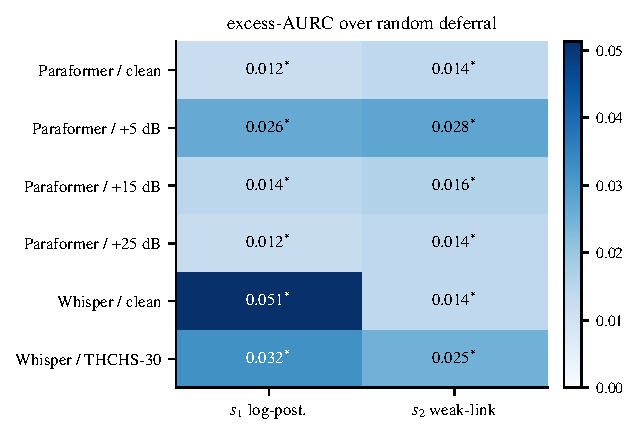
\includegraphics[width=0.65\linewidth]{fig2_holm_matrix.pdf}
  \caption{Realized $m{=}12$ audit family: excess-AURC over analytic random deferral for
  $\{s_1,s_2\}$ across six (backbone $\times$ condition) cells. Cell magnitudes are the
  informative quantity; their speaker-blocked bootstrap 95\% CIs all exclude zero
  (Holm-controlled audit family). The $^{*}$ marks the permutation rejection, which is saturated at
  the floor for every cell ($p_{\mathrm{Holm}}{=}0.006$) and hence non-discriminating.}
  \label{fig:holm}
\end{figure}

\begin{table}[t]
  \centering
  \caption{Realized audit family, $m=12$ (expansion). Excess-AURC over the analytic
  random-deferral baseline, with a speaker-blocked bootstrap 95\% CI (2{,}000 resamples,
  block $=$ speaker; computed post-hoc from the frozen scored artifacts, prereg-neutral).
  The CI excludes zero in every cell. The median-split matched-abstention permutation
  $p$-value is at the resolution floor ($5.0\times10^{-4}$, $n_{\mathrm{perm}}=2000$) for
  all twelve cells, giving $p_{\mathrm{Holm}}=0.006$ throughout --- so the $p$-values are
  non-discriminating and the effect sizes and CIs are the informative quantities. The
  Paraformer- and Whisper-clean $s_2$ excess-AURC both round to $0.0137$ but are distinct
  ($0.01368$ and $0.01370$).}
  % source files: results/expansion/holm/holm_audit_realized.json (points);
  %   results/audit_ci.json (CIs)
  \label{tab:holm}
  \begin{tabular}{lllrc}
    \toprule
    Backbone & Condition & Score & excess-AURC & 95\% CI (speaker-blocked) \\
    \midrule
    Paraformer & Aishell clean      & $s_1$ & 0.0118 & $[0.0101,\ 0.0137]$ \\
    Paraformer & Aishell clean      & $s_2$ & 0.0137 & $[0.0119,\ 0.0156]$ \\
    Paraformer & +noise 5\,dB       & $s_1$ & 0.0264 & $[0.0195,\ 0.0348]$ \\
    Paraformer & +noise 5\,dB       & $s_2$ & 0.0275 & $[0.0208,\ 0.0358]$ \\
    Paraformer & +noise 15\,dB      & $s_1$ & 0.0144 & $[0.0122,\ 0.0169]$ \\
    Paraformer & +noise 15\,dB      & $s_2$ & 0.0161 & $[0.0138,\ 0.0187]$ \\
    Paraformer & +noise 25\,dB      & $s_1$ & 0.0124 & $[0.0107,\ 0.0144]$ \\
    Paraformer & +noise 25\,dB      & $s_2$ & 0.0142 & $[0.0123,\ 0.0162]$ \\
    Whisper    & Aishell clean      & $s_1$ & 0.0513 & $[0.0462,\ 0.0567]$ \\
    Whisper    & Aishell clean      & $s_2$ & 0.0137 & $[0.0083,\ 0.0184]$ \\
    Whisper    & THCHS-30           & $s_1$ & 0.0322 & $[0.0299,\ 0.0348]$ \\
    Whisper    & THCHS-30           & $s_2$ & 0.0248 & $[0.0228,\ 0.0266]$ \\
    % source: THCHS-30 cells recomputed on the corrected 2026-07-12 full official-test
    %   re-decode (n=2495, 10 D-prefix speaker blocks; was n=1339 / 59 blocks, wrong-pool
    %   mirror split 82.7% train-speaker). Point
    %   estimates s1=0.032210, s2=0.024796 from results/expansion/holm/holm_audit_realized.json;
    %   speaker-blocked 95% CIs from results/audit_ci.json (both still exclude zero).
    %   Old 0.0291 [0.0250,0.0331] / 0.0221 [0.0179,0.0261] (n=1339) superseded. The
    %   permutation p stays at the resolution floor, so p_Holm=0.006 and the reject
    %   decision are unchanged across the whole m=12 family.
    \bottomrule
  \end{tabular}
\end{table}

\begin{table}[t]
  \centering
  \caption{Certificate specification and the macro-vs-micro caveat. G1 (LTT with the
  Bonferroni-over-grid procedure and empirical-Bernstein $p$-values) certifies accepted-set
  macro-CER; micro-CER is reported with a speaker-blocked bootstrap CI but is
  not certified. Clip frequency (CER${}>1$) is 0 on Aishell-1 test.
  The accepted-set (certified)
  row's micro-CER is a descriptive 20-reseed companion,
  not certified.}% source: results/accepted_micro_2026-07-13.json
  % frozen config knobs: procedure=bonferroni, p_value=eb
  \label{tab:cert}
  \begin{tabular}{llrr}
    \toprule
    Backbone / condition & Statistic & macro-CER & micro-CER \\
    \midrule
    Paraformer / Aishell clean (full set)   & reported & 1.98\% & 1.94\% \\
    Paraformer / +noise 5\,dB (full set)    & reported & 3.80\% & 3.74\% \\
    Paraformer / +noise 15\,dB (full set)   & reported & 2.30\% & 2.26\% \\
    Paraformer / +noise 25\,dB (full set)   & reported & 2.04\% & 2.00\% \\
    Whisper / Aishell clean (full set)      & reported & 28.06\% & 26.17\% \\
    Whisper / THCHS-30 (full set, fixed re-decode) & reported & 9.93\% & 9.95\% \\
    % source: THCHS macro 9.93% (0.09931) and micro 9.95% (0.099545) recomputed from
    %   results/expansion/scored/thchs30_whisper_scored_fixed_2026-07-12.jsonl (n=2495);
    %   macro cross-checks numbers.json expansion_audit thchs30_whisper_crosscorpus
    %   (macro_cer 0.09931); micro = total edits / total ref chars = 8077/81139 = 0.099545.
    %   Prior draft rounded 0.099545 up to 9.96%; corrected to 9.95%. Old 15.77/15.57 superseded.
    \midrule
    Paraformer / Aishell clean (accepted, $\alpha{=}2\%$) & \textbf{certified} & 1.00--1.53\% & 1.02--1.54\% \\
    % accepted-set micro-CER: descriptive companion (not certified), 20 reseeds;
    %   results/accepted_micro_2026-07-13.json (micro 1.02-1.54%, mean 1.23%).
    \bottomrule
  \end{tabular}
\end{table}

\subsection{Comparator scores and speaker-blocked robustness}\label{sec:comparator}

Two follow-up analyses on Aishell-1 test (Paraformer, $n=7{,}172$; the same four of
$7{,}176$ test utterances with degraded token-log-probability extraction, excluded-and-counted)
address the narrowness of the $\{s_1,s_2\}$ family and the
utterance-level permutation null. First, fitting the tune-side temperature that the main
standalone audit omitted makes $s_5$ auditable, and we add a learned CER-regressor $s_6$ as
an exploratory comparator. On the primary family $\{s_1,s_2,s_5\}$ (Holm $m=3$) all three
reject at $\alpha=0.05$ with excess-AURC $0.0118/0.0137/0.0118$ ($p_{\mathrm{Holm}}=0.0015$);
the exploratory $s_6$ rejects with excess-AURC $0.0125$ ($p_{\mathrm{Holm}}=0.0005$). The
$s_5$ excess-AURC equals $s_1$'s exactly because temperature scaling is order-preserving and
leaves the risk--coverage ranking unchanged --- $s_5$ buys calibration, not ranking. Second,
we re-run the matched-abstention permutation null with speaker-level blocking: for all four
scores the speaker-blocked $p$ sits at the same resolution floor ($5.0\times10^{-4}$,
$n_{\mathrm{perm}}=2000$) as the utterance-level null (\cref{tab:comparator}), so the audit
verdict does not depend on within-speaker exchangeability. The $s_1,s_2$ effect sizes match
their Paraformer-clean entries in \cref{tab:holm} (same substrate).
% source: m4_m6_audit_2026-07-12/M4-M6-RESULT.json --
%   m4.primary_audit_s1_s2_s5.results (excess_aurc s1=0.011802, s2=0.013680, s5=0.011802;
%   p_holm=0.0014993; n=7172, holm_family_size=3);
%   m4.exploratory_audit_s6.results (excess_aurc=0.012471, p_holm=0.0004998);
%   m6_permutation_nulls.{s1,s2,s5,s6}.{utterance_level,speaker_blocked}.p_value=0.0004998.

\begin{table}[t]
  \centering
  \caption{Comparator audit on Aishell-1 test (Paraformer, $n=7{,}172$). Primary family
  $\{s_1,s_2,s_5\}$ under Holm ($m=3$); $s_6$ (learned CER-regressor) is an exploratory
  comparator ($m=1$). All reject at $\alpha=0.05$. The last column gives the median-split
  matched-abstention permutation $p$ under utterance-level and speaker-blocked nulls
  ($n_{\mathrm{perm}}=2000$, floor $5.0\times10^{-4}$): blocking does not weaken the verdict.
  $s_5$'s excess-AURC equals $s_1$'s because temperature scaling is rank-preserving.}
  % source file: m4_m6_audit_2026-07-12/M4-M6-RESULT.json
  % TABLEFIX-2026-07-16 KEEP-JUSTIFIED (4 data rows, < 5): checked the source file for a
  %   hidden categorical axis to expand (per the corrected review-directive guidance
  %   preferring expansion over merge/prose) -- there is none. M4-M6-RESULT.json computes
  %   this speaker-blocked-robustness check on exactly one cell (Paraformer, Aishell-1
  %   clean); s5 needs the tune-side temperature fit and s6 the learned regressor fit on
  %   Aishell dev, both backbone/condition-specific analyses that were never run on other
  %   cells, so there is no per-corpus or per-backbone detail being "summarized away" here
  %   -- these 4 rows are the complete realized family. No natural merge partner remains
  %   either: the adjacent named-baseline table (\cref{tab:baselines}) reports a different
  %   statistic (excess-AURC only, no Holm/permutation columns) over a different axis
  %   (backbone x corpus), so forcing a merge would leave most of its cells blank. Kept
  %   as-is.
  \label{tab:comparator}
  \begin{tabular}{lrrc}
    \toprule
    Score & excess-AURC & $p_{\mathrm{Holm}}$ & perm.\ null $p$ (utt.\ / spk-blocked) \\
    \midrule
    $s_1$         & 0.0118 & 0.0015 & $5.0\times10^{-4}$ / $5.0\times10^{-4}$ \\
    $s_2$         & 0.0137 & 0.0015 & $5.0\times10^{-4}$ / $5.0\times10^{-4}$ \\
    $s_5$         & 0.0118 & 0.0015 & $5.0\times10^{-4}$ / $5.0\times10^{-4}$ \\
    $s_6$ (expl.) & 0.0125 & 0.0005 & $5.0\times10^{-4}$ / $5.0\times10^{-4}$ \\
    \bottomrule
  \end{tabular}
\end{table}

\textbf{Named confidence baselines (method-vs-method).} Published ASR work reports
excess-AURC against \emph{named} confidence estimators \citep{ravi2024teles}, so we run
the TeLeS-family baselines through the identical audit machinery on the same cells
(\cref{tab:baselines}); the class-probability and path-probability baselines descend from
the word- and utterance-level confidence-estimation lineage
\citep{qiu2021wordlevel,qiu2021deletion,swarup2019alexa}, and the learned CEM is our
implementation of that lineage's logistic confidence-estimation module, not TeLeS's own
acoustic-embedding features.
The finding is a clarification of our scope, not a horse-race win: our two primary scores
are two of these standard baselines --- min-class-probability equals $s_2$ exactly,
and length-normalized path probability equals $\exp(s_1)$ (a monotone transform, hence an
identical excess-AURC) --- and the remaining derivable baselines (mean class probability, a
learned logistic confidence-estimation module fit on the Aishell-1 dev split) match $s_1,s_2$
to within $\pm0.002$ excess-AURC on every certifying cell. No named baseline dominates ours;
the contribution is the finite-sample certificate wrapped around these confidence signals,
not a novel score. (Tsallis entropy needs the full per-token posterior distribution, which
the dumps do not carry --- the emitted-token logps are present but the full vocabulary
distribution is not --- so it is reported unavailable, not imputed.) The Aishell-1/Belle
cell also surfaces on the degraded zipformer transducer (non-certifying everywhere,
\cref{tab:landscape}): its class-probability-derived scores turn \emph{negative} while
$s_2$ and the learned CEM stay positive, a property of that backbone's mis-scaled
posteriors, disclosed verdict-symmetrically rather than dropped.

\begin{table}[t]
  \centering
  \caption{Named confidence-baseline excess-AURC on every backbone $\times$
  corpus cell computed by the standalone baseline run (Aishell-1 and MagicData),
  using the same audit machinery ($n_{\mathrm{perm}}{=}2000$).
  class-prob-min $\equiv s_2$ and lengthnorm-path-prob $\equiv \exp(s_1)$ by construction
  (identical rankings); mean class prob and the learned CEM are the genuinely distinct
  baselines. On Paraformer/Belle (the certifying backbones) all coincide with our scores
  within $\pm0.002$; on the non-certifying zipformer transducer, $s_1$/class-prob/lengthnorm
  turn negative while $s_2$/CEM stay positive (verdict-symmetric, consistent with zipformer's
  vacuous landscape certificate). Paraformer/MagicData is
  excluded wholesale (41/4{,}094, 1.0\% of rows lack a decoded score --- the family never
  computed, not imputed). MagicData capped to $n{=}4{,}094$ as in the certified landscape.
  Tsallis entropy: unavailable (no full posteriors). THCHS-30 cells are omitted:
  that baseline run predates the official-pool THCHS-30 redecode, and its THCHS-30 numbers
  sit on the superseded $n{=}1{,}339$ mislabeled-mirror pool; they are excluded rather than shown stale.}
  % source: baselines_2026-07-15/results.json (asr_gate.audit.run_audit, n_perm=2000, seed=0;
  %   per_score excess_aurc for cells paraformer_aishell, paraformer_magicdata, belle_aishell,
  %   belle_magicdata, zipformer_aishell, zipformer_magicdata -- all 6 rows below trace here).
  %   class_prob_min and lengthnorm_pathprob reproduce s2 and s1 to the printed digit. THCHS-30
  %   cells (paraformer_thchs30, belle_thchs30, zipformer_thchs30) exist in the same file but
  %   are on the pre-redecode n=1339 mirror pool (macro-CER 3.75/6.62/81.80%, vs the corrected
  %   4.07/6.99/82.15% in tab:landscape) -- deliberately excluded, see caption. Full table
  %   (incl. the excluded THCHS-30 rows, frozen and superseded) in baselines_2026-07-15/RESULTS.md.
  \label{tab:baselines}
  \small
  \setlength{\tabcolsep}{2pt}
  \begin{tabular}{l l r r r r r r r}
    \toprule
    Backbone & Corpus & macro-CER & $s_1$ & $s_2$ & class-prob & class-prob & lengthnorm & learned \\
             &        &           &       &       & (mean) & (min)$\,{\equiv}s_2$ & path$\,{\equiv}\exp s_1$ & CEM \\
    \midrule
    Paraformer & Aishell-1  & 1.98\%  & 0.0118 & 0.0137 & 0.0117 & 0.0137 & 0.0118 & 0.0122 \\
    Paraformer & MagicData  & 4.89\%  & \multicolumn{6}{c}{excluded: 41/4{,}094 (1.0\%) rows missing every score, family dropped} \\
    Belle      & Aishell-1  & 5.12\%  & 0.0236 & 0.0221 & 0.0237 & 0.0221 & 0.0236 & 0.0199 \\
    Belle      & MagicData  & 7.80\%  & 0.0420 & 0.0372 & 0.0422 & 0.0372 & 0.0420 & 0.0346 \\
    zipformer  & Aishell-1  & 45.88\% & $-$0.0158 & 0.0578 & $-$0.0226 & 0.0578 & $-$0.0158 & 0.1890 \\
    zipformer  & MagicData  & 32.21\% & $-$0.0055 & 0.0567 & $-$0.0102 & 0.0567 & $-$0.0055 & 0.1504 \\
    \bottomrule
  \end{tabular}
\end{table}

\subsection{The certified landscape: three backbones $\times$ three Mandarin corpora}\label{sec:landscape}

To move the certificate off a single (backbone, corpus) cell, we preregistered
(\textsc{freeze-amendment 2026-07-13}, signed before any new test split was touched) and
ran a frozen landscape: three backbones spanning three architectures --- Paraformer (B2,
NAR-CIF), Belle-whisper-large-v3-zh (B3$'$, attention encoder--decoder), and an offline
zipformer transducer \citep{yao2024zipformer} (B4, RNN-T) --- across three credential-free Mandarin corpora
(Aishell-1, THCHS-30, MagicData), on the frozen $\alpha$-grid $\{1.5,2,3,5,10\}\%$ with
$\delta{=}0.1$ and 20 speaker-level reseeds per cell. Each backbone's gate is calibrated
once on the Aishell-1 dev split and applied to every test split, so the THCHS-30 and
MagicData cells are cross-corpus transfer cells (reported as transfer, never
conflated with in-corpus Aishell). \Cref{fig:landscape,tab:landscape} give the certified frontier.

\begin{figure}[t]
  \centering
  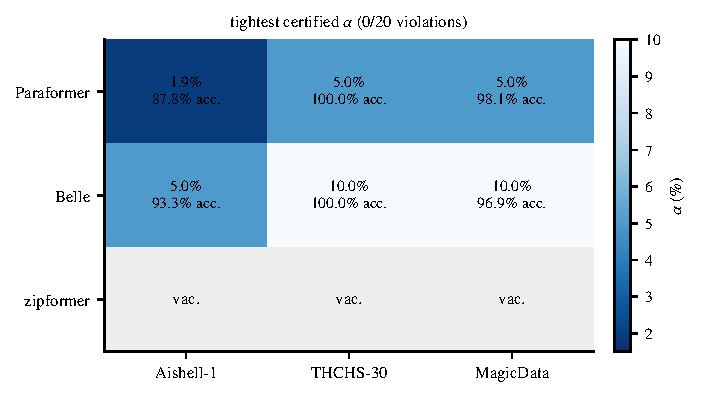
\includegraphics[width=0.72\linewidth]{fig7_landscape.pdf}
  \caption{Certified landscape: tightest non-vacuous target (20 reseeds, 0 violations) for
  three backbones $\times$ three Mandarin corpora. Cell text is that target and mean
  acceptance. Vacuous cells accept nothing. Paraformer/Aishell-1 uses the binding
  $1.9\%$ target; other cells use the frozen $\alpha$-grid.}
  \label{fig:landscape}
\end{figure}

\begin{table}[t]
  \centering
  \caption{Certified landscape (frozen protocol; 20 reseeds/cell,
  $\delta{=}0.1$). ``Tightest cert.\ $\alpha$'' is the smallest grid $\alpha$ certifying
  non-vacuously with 0/20 reseed violations; acceptance and accepted-set macro-CER are its
  20-reseed means. Aishell-1 is in-corpus (official test, $n{=}7{,}176$); THCHS-30
  ($n{=}2{,}495$, the corrected full official test---ten D-prefix test speakers,
  re-decoded 2026-07-16, disclosed as a protocol deviation) and MagicData (speaker-disjoint $\sim$4k
  eval cap, $n{=}4{,}094$) are Aishell-dev-calibrated transfer cells.
  \textsc{vac.} $=$ vacuous at every grid $\alpha$; for these rows the accept and
  acc-CER cells are \textemdash{} (no set is accepted, so both are undefined).}
  \label{tab:landscape}
  \small
  \begin{tabular}{l l r c r r}
    \toprule
    Backbone & Corpus & full-set CER & tightest cert.\ $\alpha$ & accept & acc-CER \\
    \midrule
    Paraformer (B2)  & Aishell-1  & 1.98\%  & 1.9\%\,$^\dagger$ & 87.8\% & 1.09\% \\
    Paraformer (B2)  & THCHS-30   & 4.07\%  & 5\%   & 100\%  & 4.06\% \\
    Paraformer (B2)  & MagicData  & 4.89\%  & 5\%   & 98.1\% & 4.12\% \\
    Belle (B3$'$)    & Aishell-1  & 5.12\%  & 5\%   & 93.3\% & 4.20\% \\
    Belle (B3$'$)    & THCHS-30   & 6.99\%  & 10\%  & 100\%  & 6.99\% \\
    Belle (B3$'$)    & MagicData  & 7.80\%  & 10\%  & 96.9\% & 6.70\% \\
    zipformer (B4)   & Aishell-1  & 45.88\% & \textsc{vac.} & --- & --- \\
    zipformer (B4)   & THCHS-30   & 82.15\% & \textsc{vac.} & --- & --- \\
    zipformer (B4)   & MagicData  & 32.21\% & \textsc{vac.} & --- & --- \\
    \bottomrule
  \end{tabular}
\end{table}
% source: results/numbers.json landscape block (compute_numbers.py; 45 realized / 15
%   withdrawn aidatatang cells); full-set CER from results/landscape/audit/audit_*_*.json
%   (MagicData from results/landscape/capped_magicdata_2026-07-15/audit_magicdata_*.json,
%   n=4094 cap; THCHS-30 from the official n=2495 re-decode
%   ../thchs_official_pulled_2026-07-16/{audit/audit_thchs30_official_*.json,
%   backbone_*/reseed_*/applied_thchs30_official_alpha*.json}, cross-checked bit-for-bit
%   against THCHS_OFFICIAL_DIGEST.json: para 4.07/5%/100%/4.06, belle 6.99/10%/100%/6.99,
%   zip 82.15/vac.); Paraformer/Aishell 1.9% row from alpha015_2026-07-13/results.json
%   (binding_band_sweep alpha=0.019: certified 20/20, acc 0.8780, acc-CER 0.01089).
%   $\dagger$ 1.9% is the binding sub-base-rate target; at alpha=2% acc rises to 90.7%.

\textbf{Resolution of the single-cell and contamination readings (M1, M2).} The frontier
now spans six non-vacuous, 0/20-violation certified cells across two backbones
$\times$ three corpora, not the single $\alpha{=}2\%$/Paraformer/Aishell cell --- so the
``certificate collapses to one cell'' reading (M1) no longer holds. (All six legs are on
official uncontaminated pools: the two THCHS-30 legs were re-decoded on the corrected
$n{=}2{,}495$ official test on 2026-07-16, \cref{tab:landscape,tab:deviations}, joining the
two Aishell-1 in-corpus cells and the two MagicData transfer cells, so the single-cell
reading breaks on official pools alone.) For contamination
(M2): Paraformer-large is an industrial checkpoint whose training data is undisclosed, so
Aishell-1 test contamination cannot be excluded from Paraformer alone. \emph{Belle-whisper}
answers this by independence, not assertion: it is a different architecture (AED vs.\
NAR-CIF), from a different organization, with documented training data (Aishell-1/2
train, WenetSpeech, HKUST --- test excluded), and it also certifies non-vacuously on
the Aishell-1 test split ($\alpha{=}5\%$, acceptance $93.3\%$, accepted-set macro-CER
$4.20\%$, 0/20). Simultaneous independent memorization of the Aishell-1 test split by
two backbones this different is not a credible single explanation, which bounds the
contamination card. \textbf{Verdict-symmetric caveat.} The frozen roster's fully-open
transducer (B4, whose public training data provably excludes the Aishell-1 test) was named
as the single strongest contamination answer, but it failed to expose usable posteriors
(Aishell full-set CER $45.88\%$; its length-normalized-logprob confidence $s_1$ scores a
negative excess-AURC, worse than random deferral), so B4 is vacuous at every cell and
is reported non-certifying / degraded-posterior --- exactly as the Conformer cell is. The
fully-open leg is therefore not delivered, and sub-$3\%$ certification on Aishell-1 remains
Paraformer-only; the contamination answer rests on Belle's documented-data independence.

Belle's certificate is calibration-budget-robust at $\alpha=5\%$, but not tighter
(post-hoc). Because the contamination answer rests on Belle, we ran a post-hoc
calibration-size power curve on it, mirroring the English/Mandarin sweeps' design (fixed
official Aishell-1 test as eval; vary only $n_{\mathrm{cal}}$ over the speaker-disjoint dev
pool; here $R{=}20$ budget reseeds per cell, reporting the fraction that certify
non-vacuously rather than a single-seed crossover). The reported $\alpha{=}5\%$ floor is
cheap to reach: the flat LTT bound (identical machinery to the other sweeps) certifies
$\alpha{=}5\%$ non-vacuously in $\ge90\%$ of reseeds by $n_{\mathrm{cal}}{=}2{,}000$ ---
about $4\times$ smaller than the frozen $\approx3{,}567$-utterance gate budget already in
use --- with $0$ violations anywhere on the grid. Unlike Paraformer, though, more budget
does not keep tightening the frontier: $\alpha{=}3\%$ reaches $\ge90\%$ of reseeds only at
the full $14{,}326$-utterance dev pool (accepting a low $49.9\%$ of the fixed test
at $2.51\%$ accepted-set macro-CER), and $\alpha\le2\%$ never certifies non-vacuously in
any of the $20$ reseeds at any tested budget, including the full pool. Belle's
contamination-answer certificate is therefore calibration-budget-robust at its reported
operating point, but its sub-$3\%$ ceiling looks like a backbone/score-separation limit
rather than a calibration-budget one, consistent with the sub-$3\%$-is-Paraformer-only
statement in \cref{sec:limitations}.
% source: calsize_power_2026-07-15/results.json --- headline_min_n_cal_for_cert_frac_90pct
%   (0.05->2000, 0.03->14326, 0.02->null, 0.015->null); cells n_cal=2000/alpha=0.05:
%   cert_fraction=1.0, 0 violations; cells n_cal=14326/alpha=0.03: cert_fraction=1.0,
%   mean_eval_accept_rate=0.4993, mean_eval_accepted_macro_cer=0.025114, 0 violations;
%   cells alpha in {0.015,0.02}: cert_fraction=0.0 at every n_cal in the grid (up to and
%   incl. 14326, the full dev pool). Same flat LTT/EB/Bonferroni machinery (delta=0.1,
%   n_grid=200, min_accept_frac=0.1) as english_calsweep_2026-07-13 /
%   mandarin_calsweep_2026-07-13; consistency_guard reproduces_frozen=true (max|ds1|=
%   max|dCER|=0.0 over 7,176 utts).

\section{Discussion}\label{sec:discussion}

The two claims are deliberately separable. C1 is a guarantee whose usefulness is
contingent on the backbone: it is informative on Paraformer (error cut by roughly $40\%$
at 91\% coverage), robust to moderate noise, and honestly vacuous on a backbone whose
floor CER exceeds the target. C2 is a debunking test that survives independently of C1
--- it confirms, across a broad realized family, that field-standard ASR confidence is
not merely random, which is the precondition any selective deployment implicitly
assumes yet is seldom tested directly \citep{traub2024selective}. Relative to \citet{ernez2023conformal} we
certify an accept/defer decision's population risk rather than the WER of a prediction
set; relative to generic non-monotone risk control
\citep{angelopoulos2026nonmonotone,yu2026joint} we contribute the ASR instantiation,
the random-deferral audit, and the Mandarin/CER evidence, not new machinery. The
apparatus (analytic random-deferral excess-AURC, matched-abstention null,
speaker-blocked bootstrap, conformal gate) transplants from selective classification
and off-policy evaluation to sequence-output ASR with only the LTT layer added.
Distribution-free risk control has been deployed analogously elsewhere:
\citet{fisch2022limitedfp} bound false positives in multi-label conformal sets,
\citet{schuster2022calm} calibrate an early-exit stopping rule for autoregressive
decoding under a similar Learn-then-Test-style guarantee, and \citet{tibshirani2019covariateshift}
extend conformal validity under covariate shift --- the same distributional-drift
concern our domain fingerprint flags rather than resolves (\cref{sec:honest}).

\section{Limitations}\label{sec:limitations}

The certificate's tightest ($\le3\%$) statement rests on one backbone (Paraformer): the
documented-data Belle backbone certifies on Aishell-1 test only at $\alpha\ge5\%$ (a
post-hoc calibration-size power curve shows this floor is calibration-budget-robust ---
non-vacuous in $\ge90\%$ of $20$ reseeds by $n_{\mathrm{cal}}{=}2{,}000$ --- but
$\alpha\le2\%$ never certifies even at the full $14{,}326$-utterance dev pool, so the
floor past $\alpha{=}3\%$ looks like a backbone/score limit, not a budget one), the
fully-open zipformer failed to expose usable posteriors and certifies nowhere, and the
Conformer-Aishell/Whisper cells are degraded-excluded or vacuous (\cref{sec:landscape}).
So while the landscape breaks the single-cell reading, the sub-$3\%$ regime is still
Paraformer-only. Scores $s_3,s_4$ are structurally null on Paraformer (no $N$-best margin or
full posteriors); $s_5$ becomes auditable only once the tune-side temperature is fit, and
a learned $s_6$ is reported as an exploratory comparator (\cref{sec:comparator}). The main
run's $m=2$ Holm family is nearly toothless; the multiplicity claim rests on the
expansion's $m=12$. Twenty test speakers give only 20 blocks for the speaker-blocked
bootstrap, so those intervals are wide by construction (the audit's permutation verdict,
however, is unchanged under speaker-level blocking, \cref{sec:comparator}). The certificate
is on macro-CER; micro-CER is reported, not certified. The cross-lingual English certificate
is non-vacuous at $\alpha=5\%$ on the frozen $613$-utterance carve and vacuous at
$\alpha\le3\%$ there; a post-hoc calibration-size sweep shows this sub-$5\%$ vacuity is a
calibration-budget effect, $\alpha=3\%$ (and $\alpha=2\%$ on the strongest backbone) becoming
certifiable at a larger calibration budget (\cref{sec:crosslingual}). The Mandarin
cross-corpus certificate that an earlier draft flagged as the highest-value follow-up is now
delivered: Paraformer and Belle both certify non-vacuously as transfer cells on MagicData and
on THCHS-30 (\cref{sec:landscape}); the two THCHS-30 legs were re-decoded on the corrected
$n{=}2{,}495$ official test (\cref{tab:deviations}), so both MagicData and THCHS-30 are
uncontaminated cross-corpus transfer legs. All results are on read Mandarin and
English plus additive-noise and cross-corpus stress; spontaneous-speech robustness is
untested. Broader Mandarin corpora exist beyond our credential-free three --- AISHELL-2's
industrial-scale 1000-hour read corpus \citep{du2018aishell2} and WenetSpeech's
10000+-hour multi-domain web/podcast collection \citep{zhang2022wenetspeech} --- both
requiring heavier licensing or download infrastructure than the SLR-hosted corpora used
here; extending the landscape to spontaneous, multi-domain Mandarin speech is exactly the
corpus axis WenetSpeech would add, left for future work.

\section*{Data \& Code Availability}
Code and archived experimental artifacts will be released in a public
repository and archived under a DOI for reproduction
% TODO-USER: insert the repository URL and Zenodo DOI before submission
so that every figure and table regenerates from those records.
The noise corpus (ESC-50, CC BY-NC family) is used as data
only; no CC-BY-NC code or weights are executed anywhere in the pipeline. MagicData (SLR68,
CC BY-NC-ND 4.0) is likewise consumed as evaluation data, not redistributed: what we archive
are derived per-utterance CER metrics, not the audio or transcripts, so the
no-derivatives term is respected (no adapted corpus is shared); if a stricter reading of ND
is preferred, the Apache-2.0 corpora (Aishell-1, THCHS-30) alone already deliver the
non-vacuous cross-corpus landscape, and MagicData can be dropped without disturbing any
frozen choice. For frozen-artifact
integrity we keep the original result filenames, which still carry the MUSAN SNR labels
even though the realized noise corpus is ESC-50: this is the disclosed MUSAN$\to$ESC-50
substitution (\cref{tab:deviations}), and the filenames are preserved unchanged rather than
renamed post hoc.
% released code: compute_numbers.py (number registry), figures/make_figures.py;
%   original noise result filenames read musan5db/15db/25db despite ESC-50 audio

\FloatBarrier
\bibliographystyle{plainnat}
\bibliography{refs}

\end{document}
